\documentclass[a4paper,10pt] {article}
\usepackage{graphicx}
\begin {document}
\section{Yocto Image}
\subsection{Einführung}

	Kevin und Stephan haben während diesem Projekt das Thema Yocto Image bearbeitet. Dabei sollten wir mit Hilfe von Yocto ein Image erstellen, welches eine Linux Distribution und die, von 
	vorherigen Gruppen erstellte, Anwendungssoftware des FHF-Trains.
	Allerdings hat die Linux Distribution wegen des Linux Kerns nicht funktioniert, weshalb wir uns dafür entschieden haben, nur ein RootFile-System mit der Anwendungssoftware zu erstellen,
	welche dann auf den FHF-Train übertragen wird.

\subsection{Definition Yocto}

	Das Yocto Projekt ist ein Open Source Werkzeug, welches für Entwickler von embedded Linux Systeme geschaffen wurde. Das Ziel von Yocto ist es, durch Einfügen und Ausschliessen
	gewählter Komponenten ein Linux System zu erstellen, welches von dem Nutzer auf das Endgerät angepasst wird. Um das alles zu ermöglichen, benutzt Yocto hauptsächlich BitBake und
	Open Embedded. Dafür haben wir Poky verwendet, welches uns ermöglicht den Kern, den bootloader und ein RootFile-System zu erstellen.
	
\subsection{Definition BitBake}
	
	BitBake ist ein Tool, welches in Metadaten gegebene Aufgaben ausführt. Diese Metadaten werden in BitBake-spezifischen Dateien gespeichert. Dazu gehören Rezepte (.bb),
	Konfigurationsdateien (.conf), Klassen (.bbclass) und Append Dateien (.bbappend). Append Dateien erweitern Rezepte, die den gleichen Namen besitzen. Diese Dateien werden in
	'layer.conf'-Dateien aufgelistet und werde durch eine 'bblayers.conf' an  BitBake referenziert.

	Es gibt verschiedene BitBake Befehle, die einem erlauben, aus den oben genannten Dateien ein Image zu erstellen. Dazu gehören:
	\begin{itemize}
	\item core-image-minimal: Das kleinste mögliche Image, welches dem Zielsystem erlaubt die Kommandozeile zu booten.
	\item core-image-base: Ein Image, welches core-image-minimal durch Hardwareunterstützung wie beispielsweise W-LAN und Bluetooth erweitert.
	\item core-image-full-cmdline: Dieses Image erweitert minimal durch Kommandozeilen-Befehle.
	\end{itemize}

\subsection{OpenEmbedded}
	Open Embedded ist eine atomatisiertes build Framework und eine Cross-Compiling Umgebung. Diese Umgebung ermöglicht es Maßgeschneiderte Linux Images für eingebettete Systeme 
	zu erstellen.
	\\ \textbf {muss noch weiter erläutert werden}
	\newpage

\subsection{Hob}
	Hob ist ein BitBake User Interface, welches das Erstellen der Images vereinfacht. Über Hob kann man einfach das Zielsystem und den BitBake-Befehl auswählen. Wenn man eine eigene
	Layer-Datei erstellt hat, kann man diese auch der Liste der aktuellen Layers hinzufügen. Des Weiteren bietet Hob eine komplette Liste von Paketen, die in den Layers aufgeführt sind 
	und lässt den User auswählen, welche er installieren möchte. Nach den Einstellung startet Hob den BitBake-Befehl und erstellt eine Image Datei.

\section{Ablauf Yocto}
\subsection{Erstellung einer virtuellen Maschine}
Um Yocto benutzen zu können mussten wir zur aller erst eine virtuelle Linux Maschine erstellen Yocto nur auf einem Linux basierten Betriebssystem funktioniert. Die folgenden Betriebssysteme wurden von den Entwicklern getestet und als stabil bezeichnet:
	\begin{itemize}
	\item Ubuntu 12.04 (LTS)
	\item Ubuntu 13.10
	\item Ubuntu 14.04 (LTS)
	\item Fedora release 19 (Schrödinger's Cat)
	\item Fedora release 20 (Heisenbug)
	\item CentOS release 6.4
	\item CentOS release 6.5
	\item Debian GNU/Linux 7.x (Wheezy)
	\item OpenSUSE 12.2
	\end{itemize}
Da wir mit Ubuntu bis jetzt am meisten Erfahrung hatten, haben wir uns recht schnell dafür entschieden Ubuntu 14.04 (LTS) zu benutzen.

\newpage
\subsection{Yocto Installation}

Sobald wir mit der Erstellung einer virtuellen Maschine fertig waren mussten wir uns um die Installation vom Yocto Projekt kümmern.
Um Yocto (bzw. Poky) zu installieren mussten wir zuerst die folgenden Pakete mittels der Kommandozeile „apt-get install“ installieren:
	\begin{itemize}
	\item gawk 
	\item wget 
	\item git-core 
	\item diffstat 
	\item unzip 
	\item texinfo 
	\item gcc-multilib 
	\item build-essential 
	\item chrpath 
	\item socat 
	\item cpio 
	\item python 
	\item python3 
	\item python3-pip
	\item python3-pexpect 
	\item xz-utils 
	\item debianutils 
	\item iputils-ping 
	\item libsdl1.2-dev 
	\item xterm
	\end{itemize}
Danach haben wir im Homeverzeichnis einen „Yocto“ Ordner angelegt indem wir mittels der Kommandozeile „git clone git://git.yoctoproject.org/poky --branch daisy“ den source Code vom Yocto Projekt heruntergeladen haben.


\subsection{Erstellung eines einfachen Images}
Mit Hilfe der Kommandozeile 'source poky/oe-init-build-env' wird es schließlich möglich Poky zu benutzen. Poky benutzt 'BitBake' um aus 'Rezpeten', Images zu machen. Bitbake ist im Grunde genommen ein Make Werkzeug das andere Make Werkzeuge (wie die, die wir ganz am Anfang installiert haben) benutzt um das Image zu bauen. 
Wir haben uns entschieden zuerst ein einfaches Image zu bauen mit Hilfe vom core-image-minimal Rezept. Dieses baut ein einfaches und leeres Root Filesystem, das eigentlich zum Testen und entwickeln von Kernels und Bootloaders gedacht ist. Um dies zu bewerkstelligen haben wir die Kommandozeile 'bitbake core-image-minimal' benutzt.
Da wir den BitBake allerdings auf einer virtuellen Maschine und nicht auf einem nativen Linux Betriebssystem haben laufen lassen hat er um die 12 Stunden gedauert (auf einem nativen Betriebssystem soll der BitBake zwischen 3 und 4 Stunden dauern).
Als das Image gebaut war konnten wir es mit Hilfe von der Kommandozeile 'runqemu qemux86' emulieren.

\subsection{Erstellung eines Root Filesystems mit Hob}
Poky bietet ein graphisches User Interface namens „Hob“ an das den BitBake Prozess übersichtlicher für den Benutzer macht:
\\\\
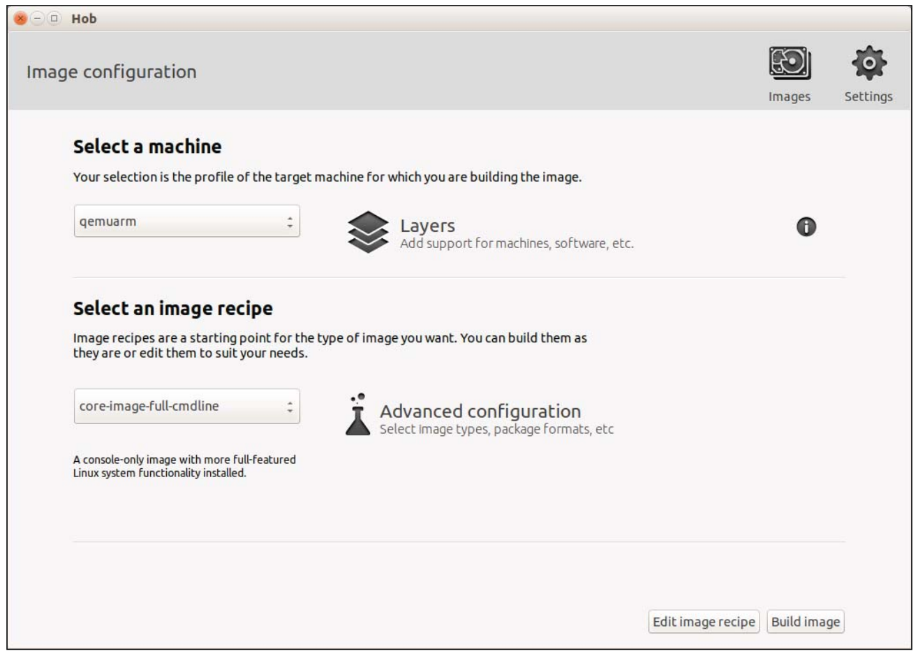
\includegraphics[width=1.0\textwidth]{Hob_Interface}
\\
\newpage
Mit Hilfe von Hob kann man dann ganz einfach eine ziel Maschine und ein Rezept aussuchen.
\\\\
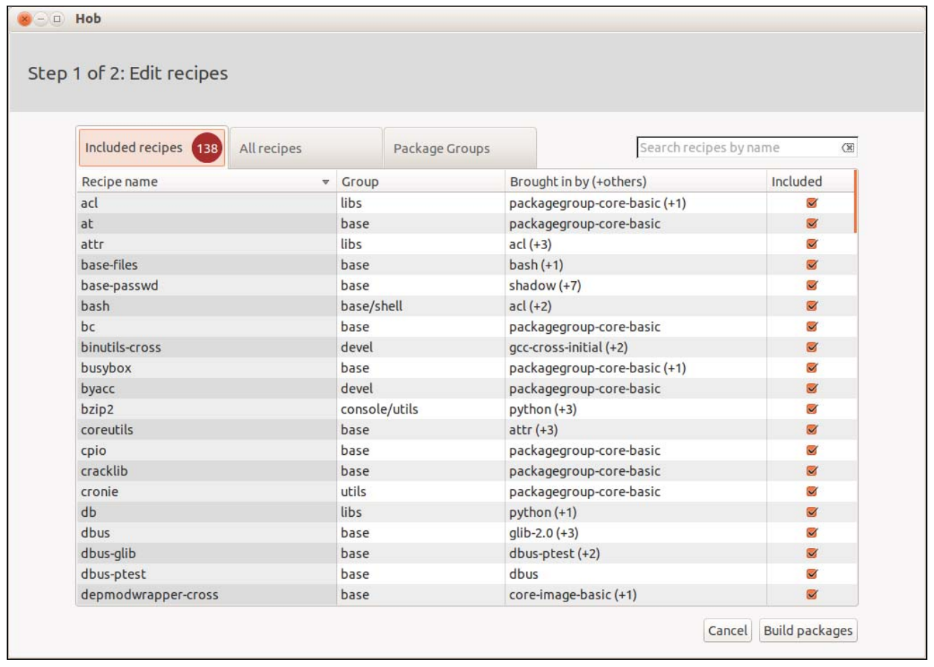
\includegraphics[width=1.0\textwidth]{Hob_Package_1}
\\\\
Danach kann man sogar wählen welche Pakete das Image braucht und welche nicht.
\\\\
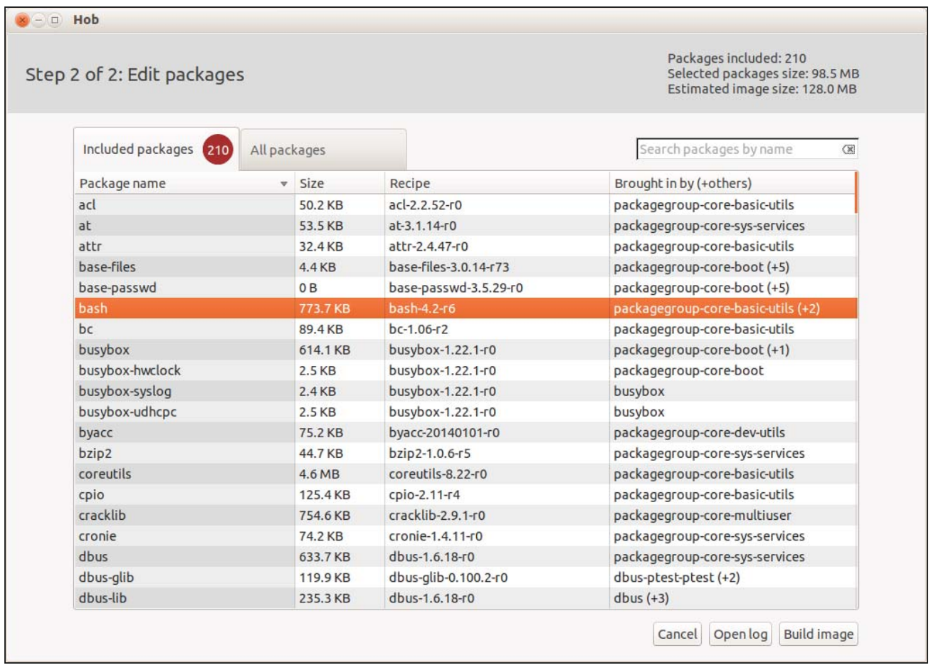
\includegraphics[width=1.0\textwidth]{Hob_Package_2}
\\\\
Nach dem auswählen der Pakete kann der Build des Images beginnen.
\\\\
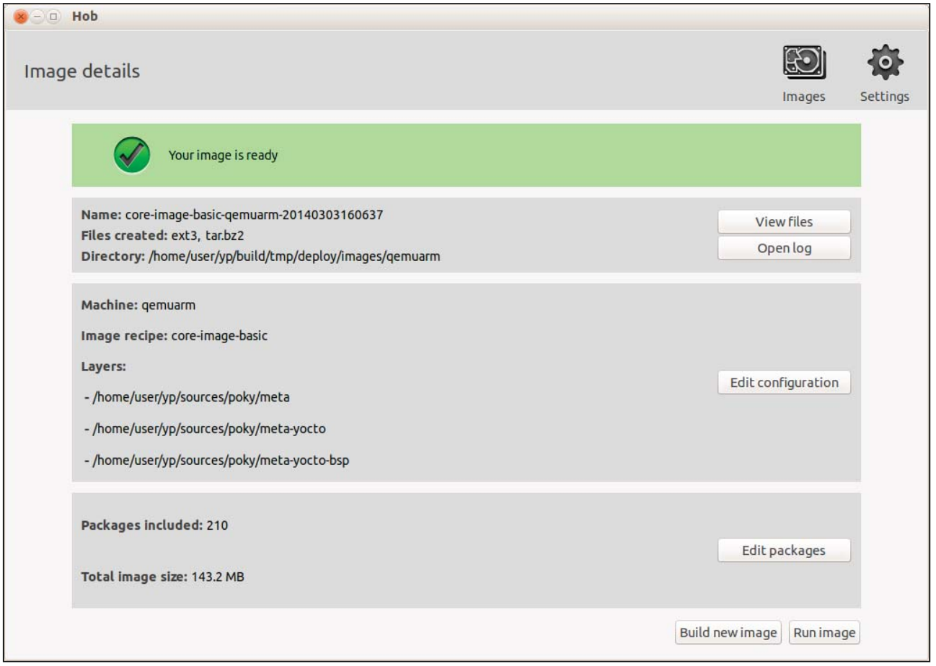
\includegraphics[width=1.0\textwidth]{Hob_Finished}
\\\\
Wenn der Build dann zu Ende ist kann das Image emuliert werden:
\\\\
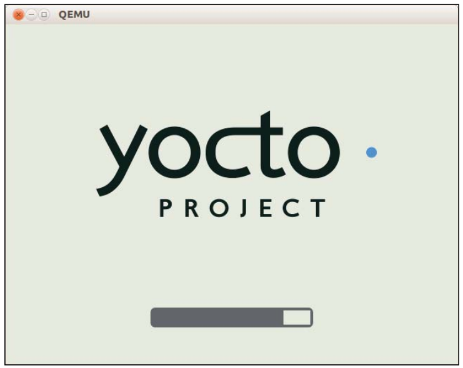
\includegraphics[width=1.0\textwidth]{Yocto_Emule}

\end {document}